
\begin{flushleft}
	\begin{enumerate}
		\item \textbf{/} 
		\begin{itemize}
			\item "/" is \textbf{top most directory} or \textbf{root directory} or \textbf{starting point} of FHS. 
		\end{itemize}
		\item \textbf{/home}
		\begin{itemize}
			\item Contains \textbf{home folder for each user} having their personal data \& configuration files.
			\item Eg: Home directory for user \textbf{jack} is \textbf{/home/jack}.
			\begin{figure}[h!]
				\centering
				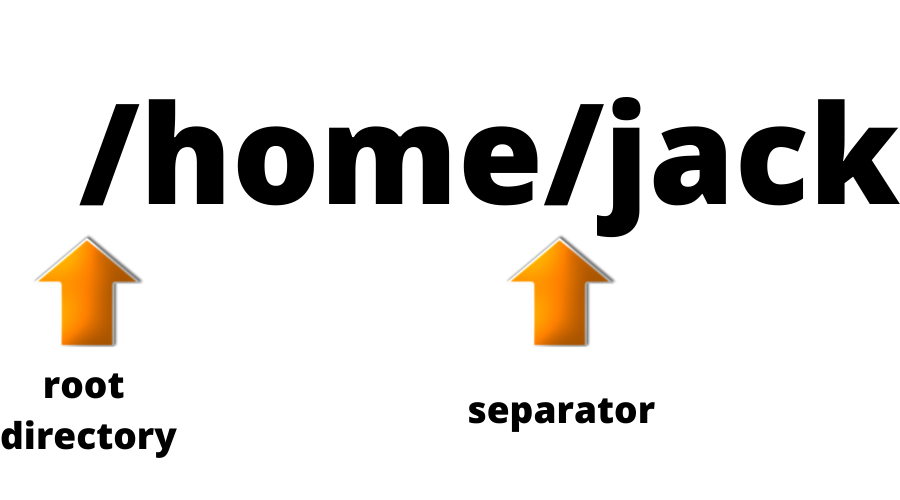
\includegraphics[scale=.3]{content/chapter2/images/path.png}
				\caption{Path separator}
				\label{fig:path}
			\end{figure}
			\begin{tcolorbox}[breakable,notitle,boxrule=-0pt,colback=yellow,colframe=yellow]
				\color{black}
				\textbf{Note:}
				\begin{itemize}
					\item Symbol \textbf{"$\sim$"} refers to the user's home directory.
					\item Eg: If you are logged in as user \textbf{"jack"}, then \textbf{"$\sim$"} meant \textbf{"/home/jack"}.
					\item Eg: If you are logged in as user \textbf{"jill"}, then \textbf{$\sim$} meant \textbf{"/home/jill"}.
					\end{itemize}
			\end{tcolorbox}
			
		\end{itemize}
		\item \textbf{/bin}
		\begin{itemize}
			\item Contains user binaries (programs).
			\item Eg: cp, mkdir, pwd, ls, rmdir etc.
		\end{itemize}
		\item \textbf{/sbin}
		\begin{itemize}
			\item Contains system administration binaries.
			\item Eg: fdisk, useradd, userdel, ifconfig etc.
		\end{itemize}
	\newpage
		\item \textbf{/usr}
		\begin{itemize}
			\item Contains read-only commands, libraries and data.
			\begin{itemize}
				\item \textbf{/bin} is link to \textbf{/usr/bin}
				\item \textbf{/sbin} is link to \textbf{/usr/sbin}
				\item \textbf{/lib} is link to \textbf{/usr/lib}
			\end{itemize}
		\end{itemize}
		\item \textbf{/etc}
		\begin{itemize}
			\item Contains system-wide configuration files.
			\item Eg: 
			\begin{itemize}
				\item /etc/fstab
				\item /etc/sysconfig/network-script/
			\end{itemize}
		\end{itemize}
			\item \textbf{/opt}
			\begin{itemize}
				\item Opt stands for optional.
				\item Used by proprietary 3rd party software to store their settings.
			\end{itemize}
		\item \textbf{/tmp}
		\begin{itemize}
			\item Contains temporary files of system.
			\item Files under this are deleted when system is rebooted.
		\end{itemize}
		\item \textbf{/var}
		\begin{itemize}
			\item Var stands for variable files.
			\item /var includes:
			\begin{itemize}
				\item System log files: \textbf{/var/log}
				\item Packages and database files: \textbf{/var/lib}
				\item Emails: \textbf{/var/mail}
				\item Lock files: \textbf{/var/lock}
				\item Temporary files needed across reboots: \textbf{/var/tmp}
			\end{itemize}
		\end{itemize}
			\item \textbf{/mnt}
		\begin{itemize}
			\item Temporary mount directory.
		\end{itemize}
		\item \textbf{/boot}
		\begin{itemize}
			\item Contains grub2 bootloader, kernel, initramfs etc. needed during system boot up.
		\end{itemize}
		\item \textbf{/media}
		\begin{itemize}
			\item Mounts temporary media device like USB drive.
		\end{itemize}
	\newpage
		\item \textbf{/proc}
		\begin{itemize}
			\item Contains running process informations.
			\item Eg: /proc/\{pid\} directory contains information about the process with that particular process.
		\end{itemize}
		\item \textbf{/run}
		\begin{itemize}
			\item Used for run-time variable data.
			\item Eg: Socket files, Process IDs etc.
			\item Difference between \textbf{/run} \& \textbf{/tmp}:
			\begin{itemize}
				\item Data in \textbf{/run always get deleted at next boot}
				\item Data in /tmp may or may not get deleted at next boot.
			\end{itemize}
		\end{itemize}
	\end{enumerate}
	
\end{flushleft}

\newpage
